\chapter{Software and Computing}
\label{ch:detectors-sc}

\section{Overview}

The Software and Computing effort is not part of the DUNE project and
is supported from non-project funds. This effort is coordinated by the
DUNE collaboration and across the LBNF/DUNE project. The three primary
components of the effort include the computing hardware, software
infrastructure and reconstruction.

\section{Computing Infrastructure}
\label{sec:detectors-sc-infrastructure}

%\subsection{Overview}
There are many factors that influence the
data (e.g. rates, volume, etc.) to be collected and processed in DUNE.
\anxrates\ describes the data rates and
provides a reference to the parameters and assumptions used
in the estimating these characteristics.  The Annex
contains information on both the reference design and alternative
design for the far detector.

\subsection{Raw Data Rates}
\label{sec:detectors-sc-infrastructure-data-rates}


\subsubsection{Types of data (using Supernova Burst example)}
DUNE is a multipurpose apparatus and will pursue a variety of physics
goals.  This will be reflected in different
characteristics of data streams processed and collected in real time
as well as offline and different strategies and algorithms for
handling these streams.

As one example, consider the difference between neutrino oscillation
physics with beam neutrinos on the one hand and the search for supernova
neutrino bursts on the other.  Signals produced by ``beam events''
will be characterized by total energy in the GeV range, so that
various aspects of handling the signal and the data (e.g. thresholds
for zero suppression etc) can be optimized for minimum-ionizing
particles.

The energy scale of signals produced by supernova
neutrino burst interactions is in the range of tens of MeV.
For that reason, it is expected that lower thresholds will be needed
while processing these data in real time, which will result in
considerable additional contribution from radiological backgrounds.  For this
reason, the data rate that needs to be handled in the process of
supernova neutrino bursts search can be expected to be quite
significant.

Another differentiating feature of supernova neutrino bursts is that
\textit{multiple neutrinos are expected to arrive and interact in the
  detector volume} within seconds of each other, as opposed to a
single vertex produced by a beam neutrino (or any other localized
interactions and/or decays). This opens an opportunity to apply the
DAQ architecture presented in~\ref{sec:detectors-fd-ref-daq} to make
these data ``self-triggering'', i.e.  to use the buffer memory in the
LArTPC detector readout to detect a corresponding signature in the
data stream and trigger recording of the potential supernova neutrino
burst event.

The characteristic time scale for such supernova neutrino burst data
capture will be $\sim$\SI{10}{\second}.  Given the large amount of
data arriving within this time period (see the Annex) and practical
limits on the bandwidth of the connection between the RCE data
processors and frontend computers in DAQ, local storage attached to
data processors will be necessary to record the data at full-stream
(no zero-suppression).  The buffer in the data processor will not have
sufficient capacity due to design and cost considerations (it can
effectively buffer about \SI{0.4}{\second} of streaming data which is
likely enough for the trigger decision but not for the complete
supernova event capture).  Preliminary estimates indicate that a
storage device such as a SSD (one or two per board) will have speed
sufficient for this purpose.  With trigger properly tuned, the number
of times data are written to the SSD can be kept sufficiently low so
as to ensure their longevity.  Once captured in this manner, the data
can then be transmitted to the rest of the farm within the available
bandwidth.

The core elements of the DAQ system now exist as prototypes.  The
system as a whole with capabilities such as descibed above is in the
conceptual design stage and information will be added to DUNE planning
documents as it is developed.




%This section focuses on data streams present in oscillation physics studies with beam
%neutrinos, since these data will constitute the bulk of what's committed
%to mass storage, transmitted over networks, processed offline and in general have most significant
%infrastructure and cost implications.
%Issues and parameters related to other classes of data
%are covered in ``\anxrates'', and also in the DAQ and other sections.

\subsubsection{Assumptions}
\label{sec:detectors-sc-infrastructure-assumptions}
According to the present baseline design, the Far Detector will
consist of four identical modules of \tpcmodulemass each.  For
purposes of estimating data characteristics in this document the issue
of possible variations in the design of these modules shall not be
addressed. A few basic assumptions:
\begin{itemize}
\item Estimates correspond to the ``full detector'',
  i.e. is effectively normalized to \dunedetectormass.
\item Accelerator spill cycle is \beamspillcycle with beam expected
  for \beamrunfraction of each calendar year.
\item Zero-Suppression thresholds will be set at levels that preserve
  signals from minimum-ionizing particles while effectively removing
  data due to electronics noise.
\item The DAQ will be able to trigger based on spill times and will be
  able to reject isolated $^{39}$Ar decays on at least a per-APA
  basis. (for DAQ details see~\ref{sec:detectors-fd-ref-daq})
\end{itemize}

\subsubsection{Far Detector LArTPC}
The information presented below is based on the parameters listed in
``\anxrates''.
\begin{itemize}
\item TPC channel count: \dunenumberchannels (i.e. four times the
  \daqchannelspermodule channel count for each \tpcmodulemass module)
\item Maximum drift Time: \tpcdrifttime
\item Number of drift time windows in one DAQ readout cycle: \daqdriftsperreadout
\item ADC clock frequency: $\sim$\daqsamplerate
\item ADC resolution (bits): 12
\end{itemize}

In addition to these basic parameters, there are other factors
affecting data rates and volumes, such as implementation of ero
suppression (ZS) in the DAQ RCE processors,
contribution from radiological and cosmological backgrounds, and DAQ
trigger configuration (cf. the case of low-energy events).

Non-ZS maximum event size (corresponding to a snapshot of the complete
TPC) can be calculated as a product of the following numbers:
\begin{itemize}
\item Channel count
\item Number of ADC samples per total drift (collection) time
\item Drift time windows in one DAQ cycle
\item ADC resolution
\end{itemize}

This results in a total of \dunefsreadoutsize worth of TPC data in one
readout.

Zero suppression greatly reduces the event size.  An overly
conservative estimate (leaning to the higher end of the range of
values) based on a LArSoft Monte Carlo simulation of GeV-scale events
suggests a zero-suppressed and uncompressed event size of
$\sim$\beameventsize.  After compression this event size is expected
to be $\sim$\beameventsizecompressed.  This particular simulation
employed a less than optimal schema for packing data and it is
expected that with optimization these sizes can be further reduced.

Some of the driving zero-suppressed (ZS) and full-stream (FS) annual
data volumes are summarized in Table~\ref{tab:sc-zs-summary}. It is
important to note that the numbers in the row characterizing $^{39}$Ar
are given for information only and do not represent our estimates of
actual data to be committed to mass storage.
Once DAQ-level rejection of isolated $^{39}$Ar decay events is invoked
a residual amount of data is accepted when the decay is accidentally
coincident with beam-$\nu$ activity.
The data required to record this background is reduced to 3\% of the
``with-beam-$\nu$'' estimate of table~\ref{tab:sc-zs-summary} and is
thus negligible being an order of magnitude smaller than the data
associated with the beam neutrino interactions themselves.

%%%% I think this simply restates our simple assumption that isolated
%%%% 39Ar can be killed by the DAQ.
%%%%  The "high threshold" approach makes people nervous, so I don't
%%%%  think we need to invoke it.
% There is a range of possible approaches to data volume reduction in
% real time without losing much of information due to low-amplitude
% signals, which may be important for more precise particle
% identification or in search for unusual signatures that may exist due
% to new phenomena. For example, implementation of the ``trigger
% stream'' in the DAQ system (see~\ref{sec:detectors-fd-ref-daq})
% allows to trigger on event candidates using
% ``high threshold'', while capturing data in the potential event
% without applying any threshold at all. In that case, one can estimate
% the total size of the TPC data to be collected annually by multiplying
% the predicted number of beam neutrino interactions per year (estimated
% here to be \beamrate) by the full stream event size quoted above
% (\dunefsreadoutsize).  This results in an estimate of
% \beamdatayearfs of this type of data per year.


% do not edit, this is generated by dune-params

\begin{cdrtable}[Annual data volume estimations for zero-suppressed (ZS) data from various sources.]{rrrrr}{sc-zs-summary}{Annual data volume estimations for zero-suppressed (ZS) data from various sources. An additional full-stream (FS) data estimation is given for supernova burst (SNB).}
Source & Event Rate & Event Size & Data Rate & Annual Data Volume \\ \toprowrule
$^{39}Ar$ (ZS) & \SI[round-mode=places,round-precision=1]{11.16}{\mega\hertz} & \SI[round-mode=places,round-precision=0]{150.0}{\byte} & \SI[round-mode=places,round-precision=1]{1.674}{\giga\byte\per\second} &  \SI[round-mode=places,round-precision=0]{52.8262940816}{\peta\byte}\\
all in-spill & & & & \SI[round-mode=places,round-precision=0]{158.558121686}{\tera\byte} \\
with-beam-$\nu$ & & & & \SI[round-mode=places,round-precision=0]{79.279060843}{\giga\byte} \\
\colhline
cosmic-$\mu$ (ZS) & \SI[round-mode=places,round-precision=3]{0.258947264}{\hertz} &
\SI[round-mode=places,round-precision=1]{2.5}{\mega\byte} & \SI[round-mode=places,round-precision=1]{647.36816}{\kilo\byte\per\second} &
\SI[round-mode=places,round-precision=0]{20.4289491035}{\tera\byte} \\
\colhline
beam-$\nu$ (ZS) & \SI[round-mode=places,round-precision=0]{8770.19567714}{\per\year} & \SI[round-mode=places,round-precision=1]{2.5}{\mega\byte} &
\SI[round-mode=places,round-precision=2]{0.694791666667}{\kilo\byte\per\second} & \SI[round-mode=places,round-precision=0]{21.9254891928}{\giga\byte} \\
beam-$\nu$ (FS) & \SI[round-mode=places,round-precision=0]{8770.19567714}{\per\year} & \SI[round-mode=places,round-precision=1]{24.8832}{\giga\byte} &
\SI[round-mode=places,round-precision=0]{6.915456}{\mega\byte\per\second} & \SI[round-mode=places,round-precision=0]{218.230533073}{\tera\byte} \\
\colhline
SNB cand. (ZS) & \SI[round-mode=places,round-precision=0]{12.0}{\per\year} & \SI[round-mode=places,round-precision=1]{16.74}{\giga\byte} &
\SI[round-mode=places,round-precision=0]{6365.63904105}{\byte\per\second} & \SI[round-mode=places,round-precision=0]{200.88}{\giga\byte} \\
SNB cand. (FS) & \SI[round-mode=places,round-precision=0]{12.0}{\per\year} & \SI[round-mode=places,round-precision=1]{46.08}{\tera\byte} &
\SI[round-mode=places,round-precision=1]{17.5226192958}{\mega\byte\per\second} & \SI[round-mode=places,round-precision=0]{552.96}{\tera\byte} \\
\end{cdrtable}

\subsubsection{Far Detector Photon Detector (PD)}
There are variations in the basic parameters of the Photon Detector
currently in the R\&D stage, so the numbers presented below need to be
considered as ballpark values to be made more precise at a later time:
\begin{itemize}
\item Readout channel count: \num{24000} (i.e. four times the \num{6000} channel count for each 10-kt module)
\item Trigger rate is uncertain at this point due to ongoing
  investigation; one approach assumes 1 trigger per spill cycle
\item ADC resolution (bits): 12
\item ADC digitization frequency: \SI{150}{\MHz}
\end{itemize}
It is assumed that a few dozen samples will be recorded in each
channel, and there will be zero suppression of channels with signals
below a chosen threshold, resulting in an order of magnitude reduction
of the data volume.  This results in \SI{360}{\kilo\byte} per spill
cycle, and should be considered negligible from the point of view of
requirement to data handling, compared to other data sources.

\subsubsection{Near Detector Data Rates}
The near detector is subject to an intense R\&D effort and
its parameters are being optimized at this point. The
most relevant parameters of the Fine-Grained Tracker (FGT):
\begin{itemize}
\item   Straw Tube Tracker (STT) readout channel count: \ndsstchannels
\item STT Drift Time: 120~ns
\item STT ADC clock frequency and resolution (bits): \SI{3}{\ns} intervals, 10 bit
\item ECAL channel count: \ndecalchannels
\item Muon Detector Resistive Plane Chambers (RPC) channel count: \ndmuidchannels
\item Average expected event rate per spill: \textasciitilde 1.5
\end{itemize}
Since there are large uncertainties in estimates of the detector
occupancy levels per event, broad assumptions must be made to
estimate the data rate. The current estimate (as quoted in the Near
Detector section of the ``Expected Data Rates'' Annex is
\textasciitilde \nddatarate, which translates into \textasciitilde
\SI{30}{\tera\byte\per\year}.

% Assuming that 10\% occupancy in the STT and 40 samples
%per trigger, one arrives to \textasciitilde 1MB of data per event. Under same assumption, ECAL will contribute \textasciitilde 0.25MB
%and the Muon Detector \textasciitilde  0.75MB.
%Based on these parameters, the upper limit of the ND data rate can be estimated as 1.5MB/s. This translates into \textasciitilde 45TB/year. 

\subsection{Processed Data}
\label{sec:detectors-sc-infrastructure-processed-data}
For the purposes of this document, processed data is defined as most
data which is not considered ``raw'', i.e. it's data derived from raw
(including possibly multiple stages of calibration and reconstruction)
as well as data produced as a result of Monte Carlo studies.

There are uncertainties in anticipated quantities of all of these
types of data. Table \ref{tab:sc-zs-summary} contains a range of
numbers reflecting limiting cases such as ZS vs FS.  Depending on the
exact optimum readout strategy, an annual raw data volume of
\SI{1}{\tera\byte} to \SI{1}{\peta\byte} may be collected.  Assuming
that the data will undergo a few processing stages, one can expect the
need to handle as much as \textasciitilde \SI{2}{\peta\byte} of data
annually for reconstruction and a lesser volume for final analysis
purposes.

For Monte Carlo, at the time of writing typical annual volume of data
produced has been of the order of a few tens of terabytes.  Initial
expectations are that the MC sample size for beam events will need to
be 10--100$\times$ that of the data.  With Collaboration growth
and more detailed studies (e.g. of systematics) undertaken, our
expectation is that this estimate will increase.

\subsection{Computing Model}
\label{sec:detectors-sc-infrastructure-computing-model}

\subsubsection{Distributed Computing}

Given the fact the Collaboration is large and widely dispersed
geographically, a fully distributed approach to computing is planned,
based on experience gained during the operation of the LHC
experiments. This includes not only ``traditional'' Grid technologies
in the form they were deployed during the first decade of this
century, but also more recent expansion into Cloud Computing and Big
Data methodology. This will allow the DUNE Collaboration to better
leverage resources and expertise from many of its member institutions
and improve the overall long-term scalability of its computing
platform.

DUNE will operate a distributed network of federated resources, for
both CPU power and storage capability. This will allow for streamlined
incorporation of computing facilities as they become available at
member institutions, and thus is particularly amenable to accommodate
staged construction and commissioning of the detector subsystems. A
modern Workload Management System will be deployed on top of Grid and
Cloud resources to provide computing power to DUNE researchers.

\subsubsection{Raw Data Transmission and Storage Strategy}
FNAL will be the principal data storage center for the experiment. It
will serve as a hub where the data from both the facility (e.g. beam,
target and cryogenics) and the various detector systems (far and near
detectors) are collected, catalogued and committed to mass
storage. This will obviously require transmission of data over
considerable distances (certainly for the far detector). In addition,
the DAQ systems of the far detector are being designed to be located
in the vicinity of the far detector (in the cavern), which results in
an additional step of transmitting the data from 4850L to the surface.

Raw data to be collected from the detectors in DUNE are considered
``precious'' due to the high cost of operating the both the facility at
FNAL and the detectors that are part of DUNE. This leads to three
basic design elements in the data transmission and storage chain:
\begin{itemize}
\item Buffering:
\begin{itemize}
\item Adequate buffers will be provided for the DAQ systems to
  mitigate possible downtime of the network connection between 4850L
  and the surface.
\item Buffers will be provided at the surface facility to mitigate
  downtime of the network connection between the far site and FNAL.
\end{itemize}
\item Robust transmission: data transfer needs to be instrumented with
  redundant checks (such as checksum calculation), monitoring, error
  correction and retry logic.
\item Redundant replicas: it is a common practice in industry and
  research (cf. the LHC experiments) to have a total of three copies
  of ``precious'' data, which are geographically distributed.  Such
  geographical distribution of the replicas may include countries
  other than the United States, where the data will be collected.
  This provides protection against catastrophic events (such as
  natural disasters) at any given data center participating in this
  scheme, and facilitates rebuilding (``healing'') lost data should
  such event does happen.
\end{itemize}


\subsubsection{Data Management}
\label{sec:detectors-sc-infrastructure-computing-model-data-mgt}

Data will be placed into mass storage at FNAL. Along the lines
described above, additional copies (replicas) will be distributed to
other computing centers possessing sufficient resources.  A single
additional copy does not necessarily need to reside in its entirety on
a single data center; the replicas can be ``striped'' across a few
data centers if that becomes optimal at the time of implementation of
the Computing Model. For example, consideration is given to both
Brookhaven National Laboratory and NERSC as candidates for the
placement of extra replicas.

Recent progress in network and storage technologies made possible
\textit{federation of storage} across multiple data centers located at
member institutions. In this approach, data can be effectively shared
and utilized via the network (cf. ``data in the Cloud''). One example
of an advanced system of this type of XRootD.

For data distribution, a combination of managed data movement between
sites (such as ``dataset subscription'', primarily for managed
production), and a network of XRootD servers to cache processed data
and for analysis will be used.  A file catalog and a Meta-Data system
will be required for efficient data management at scale, and an effort
will be made to leverage experience of member institutions in this
area, making an effort to reuse existing systems or design ideas where
possible.

\subsection{Computing Implications of the Dual-Phase Far Detector Design}
\label{sec:detectors-sc-alternate}
Parameters of the alternative design of the far detector (based on the
dual-phase technology) are listed in Chapter 2 of the
``\anxrates''. Here is a brief summary:
\begin{itemize}
	\item Readout channel count: 614,400 (i.e. four times the
          153,600 channel count for each 10-kt module)
	\item Drift Time: 7.5~ms
\end{itemize}
\
For the Photon Detector in the dual-phase design:
\begin{itemize}
	\item Readout channel count: 720 (i.e. four times the 180
          channel count for each 10-kt module)
\end{itemize}
\ According to some estimates listed in the Annex, the ``Full Stream''
readout will produce 16.09~GB of data for each candidate event. This is
about 65\% of the data volume in one readout cycle, in the reference
design.  Although signal processing strategies may be implemented
differently in the alternative design, it can be argued that the total
data rate will be of the same order of magnitude or less than in the
reference design.

\section{Near Detector Physics Software}
\label{sec:detectors-sc-nd-physics-software}

A longer description of the current status of the near detector
simulation and reconstruction are given in \anxreco\ with an
abbreviated summary here.

Two approaches are being  pursued for the simulation of
the DUNE near detector.  The first is a fast Monte Carlo based on
parameterized detector responses. The GENIE\cite{GENIE} generator is
used to model the interactions of neutrinos with nuclei in the
detector, and a parameterization of the achieved NOMAD reconstruction
performance is used to model the detector response.  The second
approach is a full GEANT4-based simulation, which is under
development.  The fast Monte Carlo tool is based on work done for the
far detector\cite{Adams:2013qkq} (Appendix A.3) and is capable of
rapidly evaluating the sensitivity of the detector design for a broad
variety of analyses targeting specific final states.  The full
GEANT4-based simulation and subsequent reconstruction chains will be
used to inform the parameterized responses of the fast Monte Carlo, as
well as being indispensable tools for simulating and extracting
results from the near detector.
Figure~\ref{fig:ndeventdisplaychaptersc} shows the trajectory of a
negatively-charged muon with an initial momentum of 1~GeV propagating
in the straw tube tracker, as simulated using GEANT4.
\begin{cdrfigure}[Trajectory of a 1-GeV $\mu^-$ simulated in the near detector.]{ndeventdisplaychaptersc}
{The trajectory of a 1 GeV $\mu^-$ produced by the GEANT4 simulation of the near detector's straw-tube tracker.}
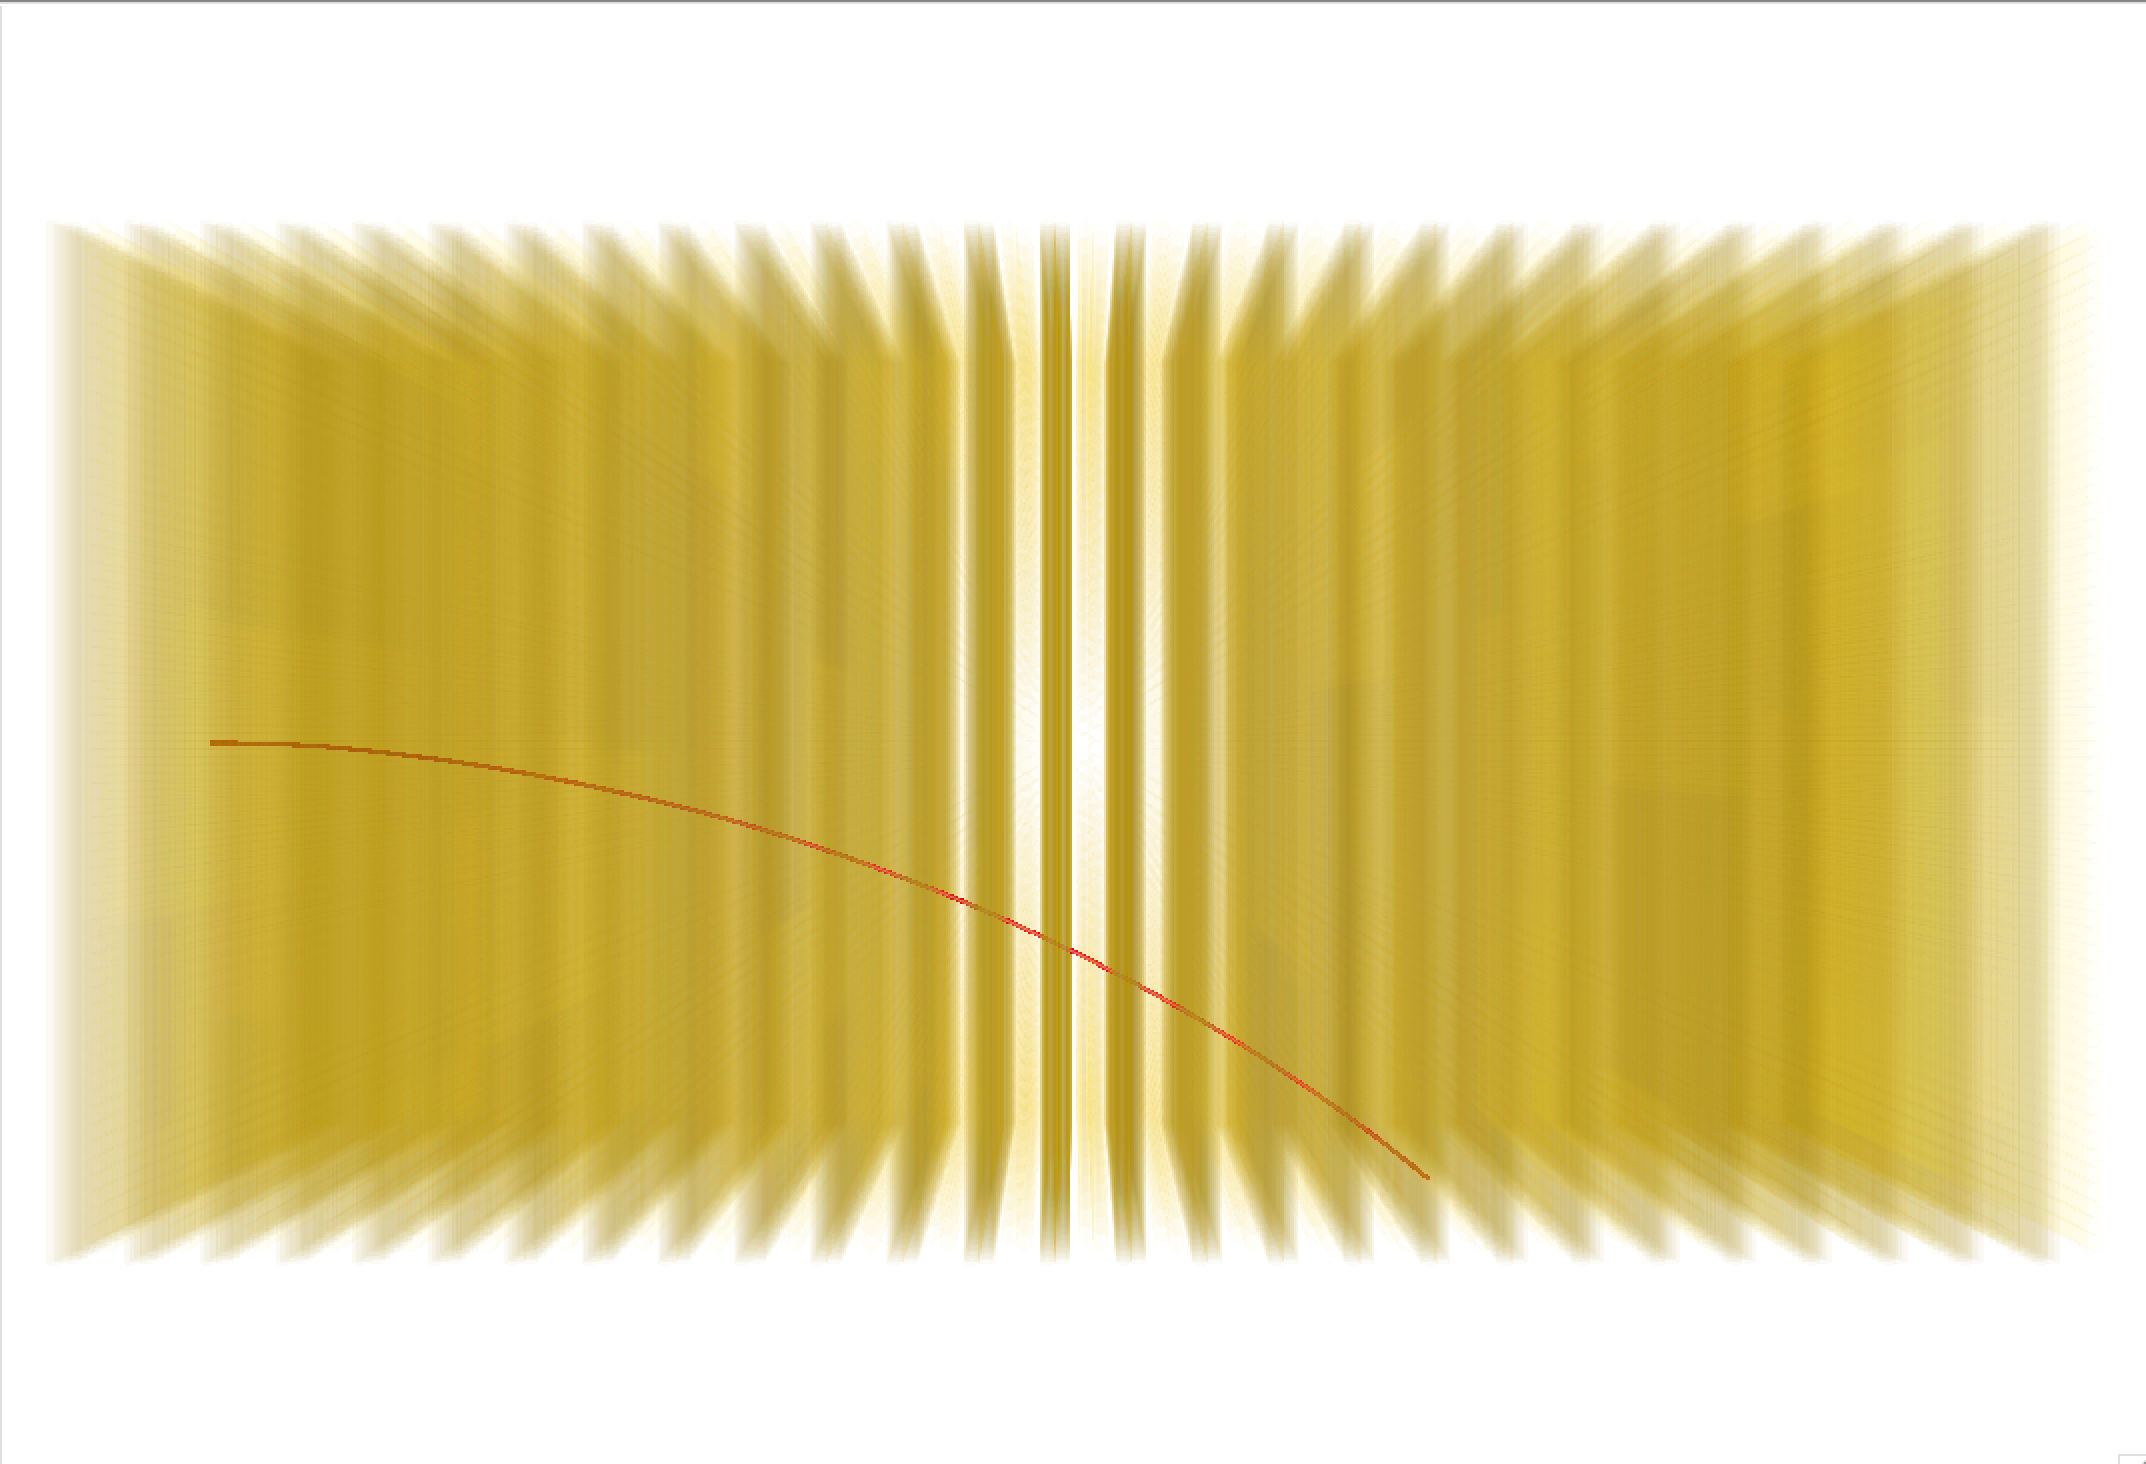
\includegraphics[width=0.7\textwidth]{hisoftndmuon.png}
\end{cdrfigure}

\section{Far Detector Physics Software}
\label{sec:detectors-sc-physics-software}

Longer descriptions of the single-phase and dual-phase far detector
simulations and reconstruction are given in \anxreco\ with an
abbreviated summary here.

%\subsection{Simulation}
%\label{sec:detectors-sc-physics-software-simulation}
% Beam simulation in the Beam Requirements chapter
%\subsubsection{Beam Simulation}
%\label{sec:detectors-sc-physics-software-simulation-beam}
% ND simulation and reconstruction in the ND chapter
%

\subsection{Far Detector Simulation}
\label{sec:detectors-sc-physics-software-simulation-fd}

Detailed GEANT4-based~\cite{GEANT4:NIM,GEANT4} Monte Carlo simulations
have been developed for the single-phase and dual-phase far detector
designs, incorporating both the TPC modules and the photon detection
systems. These simulations provide a basis for detailed studies of
detector design and performance, and also enable the development of
automated event-reconstruction algorithms.

The single-phase detector simulation is implemented in
LArSoft\cite{Church:2013hea}, which provides a common simulation
framework for LArTPC experiments.  LArSoft is based on the {\it art}
framework\cite{Green:2012gv}, and is supported by the Fermilab
Scientific Computing Division.  The comparison of data from
ArgoNeuT\cite{Anderson:2012vc,Anderson:2012mra} with LArSoft
simulations gives confidence in the reliability of the detector
simulation.  Future data from
LArIAT\cite{Adamson:2013/02/28tla,Cavanna:2014iqa},
MicroBooNE\cite{Chen:2007ae,Jones:2011ci,microboonecdr}, and the
35-ton prototype (Sec.~\ref{sec:proto-35t}) will allow further tuning
of the LArSoft simulation as experience is gained.  The dual-phase
detector simulation and hit-level reconstruction are based on the
Qscan\cite{lussi:thesis} package, which has been developed over the
past decade, and is currently being used for technical design and
physics studies for the \cerndualproto{} program.

Events are generated using either the GENIE\cite{GENIE} simulation of
neutrino-nucleus interactions, the
CRY\cite{Cosmic-CRY,Cosmic-CRY-protons,CRY-url} cosmic-ray generator,
a radiological decay simulator written specifically for LArSoft using
the decay spectra in Ref.~\cite{docdb-8797}, a particle gun or one of
several text-file-based particle input sources. GEANT4 
simulates the trajectories of particles and their energy
deposition.  Custom algorithms have been developed to propagate the
drifting charge and scintillation photons through the detector and to
simulate the response characteristics of the TPC wires, readout
electronics and photon detectors.
Figure~\ref{fig:larsofteventdisplays} shows some examples of simulated
accelerator neutrino interactions in the MicroBooNE detector.
\begin{cdrfigure}[Simulated neutrino interactions in MicroBooNE]{larsofteventdisplays}
{Examples of accelerator neutrino interactions, simulated by LArSoft
  in the MicroBooNE detector. The panels show 2D projections of
  different event types.  The top panel shows a $\nu_{\mu}$
  charged-current interaction with a stopped muon followed by a decay
  Michel electron; the middle panel shows a $\nu_{e}$ charged-current
  quasi-elastic interaction with a single electron and proton in the
  final state; the bottom panel shows a neutral-current interaction
  with a $\pi^{0}$ in the final state that decayed into two photons
  with separate conversion vertices.}
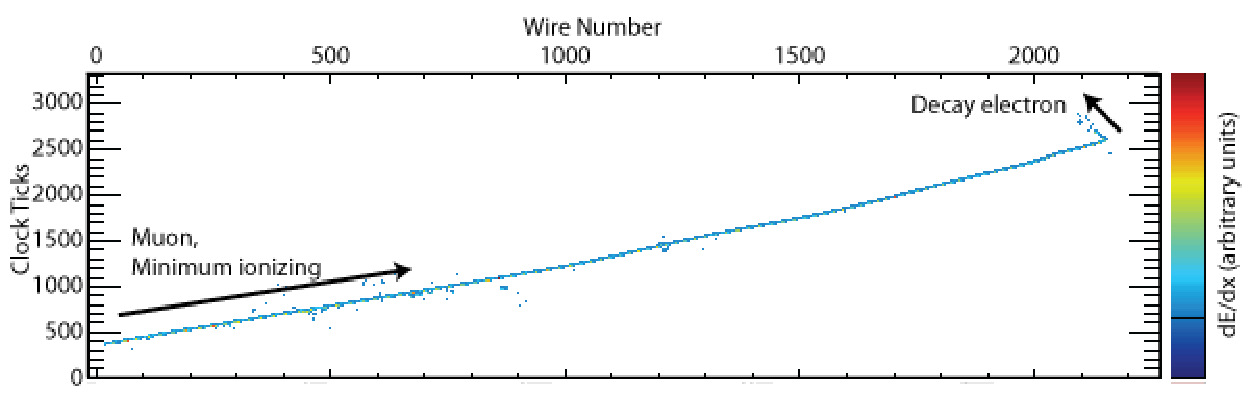
\includegraphics[width=\textwidth]{numuCC_annotated.pdf}
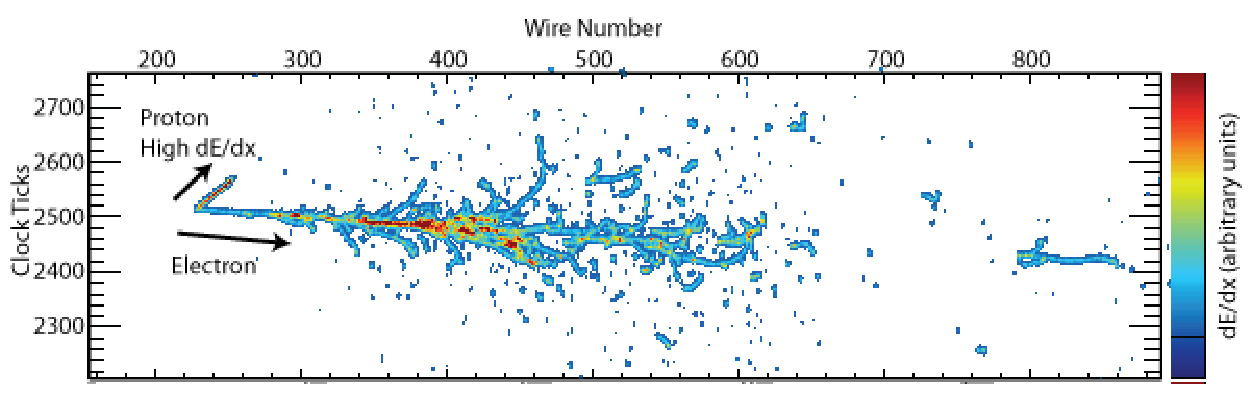
\includegraphics[width=\textwidth]{nueQE_annotated.pdf}
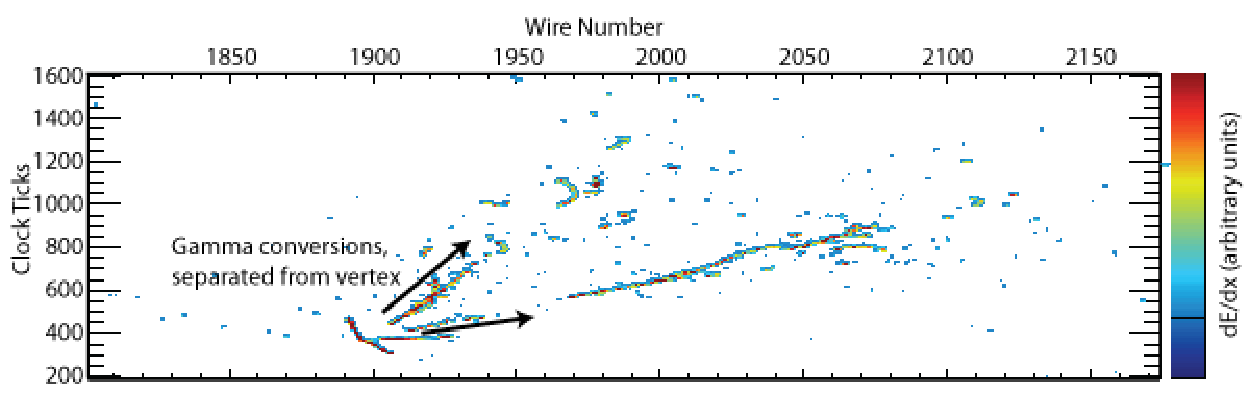
\includegraphics[width=\textwidth]{nc_pi0sep_annotated.pdf}
\end{cdrfigure}

\subsection{Far Detector Reconstruction}
\label{sec:detectors-sc-physics-software-reconstruction-fd}

The reconstruction of particle interactions in LArTPC detectors is an
active area of research that has advanced significantly in recent
years.  In particular, the analysis of the data from the
ICARUS\cite{Amerio:2004ze,icarus-url,ICARUS-pizero,Antonello:2012hu}
and ArgoNEUT
experiments\cite{Adamson:2013/02/28tla,argoneut-url,Acciarri:2013met}
required the development of a variety of new reconstruction
techniques, forming the basis for precision neutrino physics
measurements.  Accurate reconstruction is needed not only of neutrino
scattering events from the beam, but also atmospheric neutrino events,
supernova burst neutrino interactions and nucleon decay events, each
with its own requirements.  With the advance of both single-phase and
dual-phase technologies and expansion of the experimental program to
include MicroBooNE\cite{Chen:2007ae,microboone-url}, the 35-ton
prototype and the CERN test experiments, the reconstruction tools have
grown in both volume and sophistication, supported by powerful
software frameworks such as LArSoft and Qscan.

Fully automated chains of event-reconstruction algorithms are being
developed for the DUNE far detector, for both the single-phase and
dual-phase designs.  The first stage of reconstruction involves the
processing of the ADC wire signals and the identification of pulses,
or ``hits'' in the two-dimensional space of wire number and charge
arrival time.  These hits provide the input for a series of
pattern-recognition algorithms, which form 2D and 3D clusters,
representing individual particle tracks and showers.  A set of
high-level algorithms is used to reconstruct the 3D vertex and
trajectory of each particle, identify the type of particle and
determine the four-momentum.  While each stage of the reconstruction
chain has been implemented, the algorithms -- in particular those
addressing the higher level aspects of reconstruction such as particle
identification -- are rather preliminary and are in active
development.



\subsubsection{TPC Signal Processing, Hit Finding, and Disambiguation}

The signal-processing steps in the single-phase and dual-phase
detectors are similar but are accomplished with separate software.
Both proceed first by decompressing the raw data and filtering the
noise using a frequency-based filter.  The single-phase
signal-processing algorithm also deconvolves the detector and
electronics responses at this step.  Both the single-phase and
dual-phase hit-finding algorithms then subtract the baselines and fit
pulse shapes to the filtered raw data.  The hit-finding algorithms are
able to fit multiple overlapping hits.  The main parameters of the
hits are the arrival time, the integrated charge, and the width.  A
raw ADC sum is also retained in the description of a hit, which often
carries a better measurement of the total charge.  The current
algorithms are found to perform well in ArgoNeuT
analyses\cite{Anderson:2012vc} for the single-phase software and
during several phases of R$\&$D and prototyping on small-scale
dual-phase LAr-LEM-TPC
setups\cite{Badertscher:2008rf,Badertscher:2012dq}.
Figure~\ref{fig:lbnoeventdisplay} shows example event displays of the
reconstructed hits in both real and simulated data.

\begin{cdrfigure}[Dual-phase LArTPC-reconstructed events for data and MC]{lbnoeventdisplay}
{
%Badertscher:2012dq
Dual-phase LArTPC-reconstructed events for data and MC.  Top: Cosmic
ray event displays for an hadronic shower candidate.  Bottom:
Reconstructed hits for a MC simulation of a 5 GeV $\nu_{\mu}$
interaction.  The secondary particles produced in the two interactions
are distinguished with different colors based on the MC truth
information (blue=muon, green=electron, red=proton, cyan=pion).  From
Ref.\cite{Badertscher:2012dq}.  }
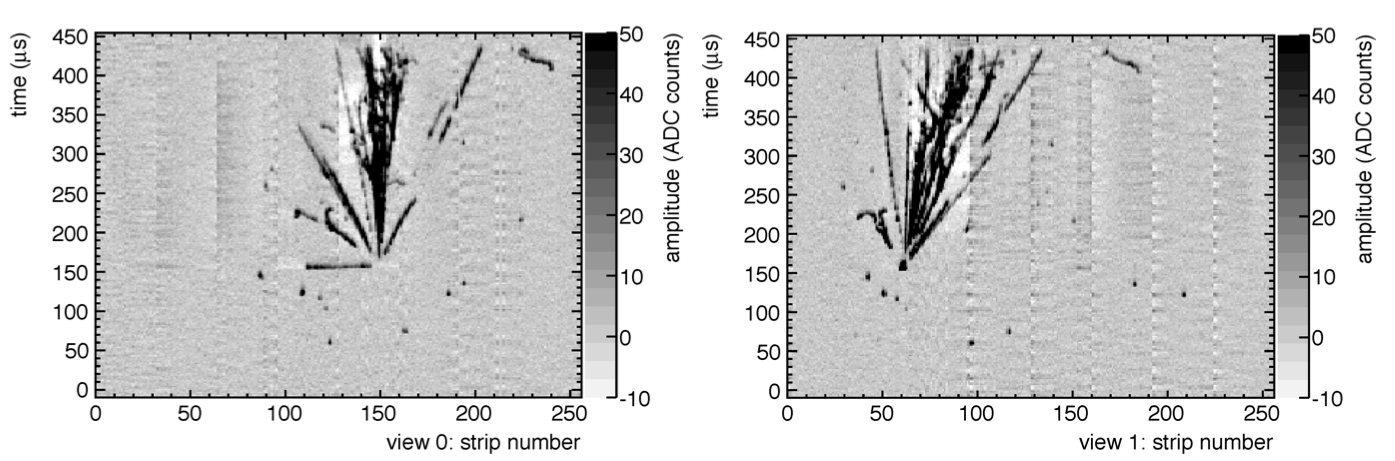
\includegraphics[width=0.99\textwidth]{LArTPC-3L-LEM-cosmics.png}
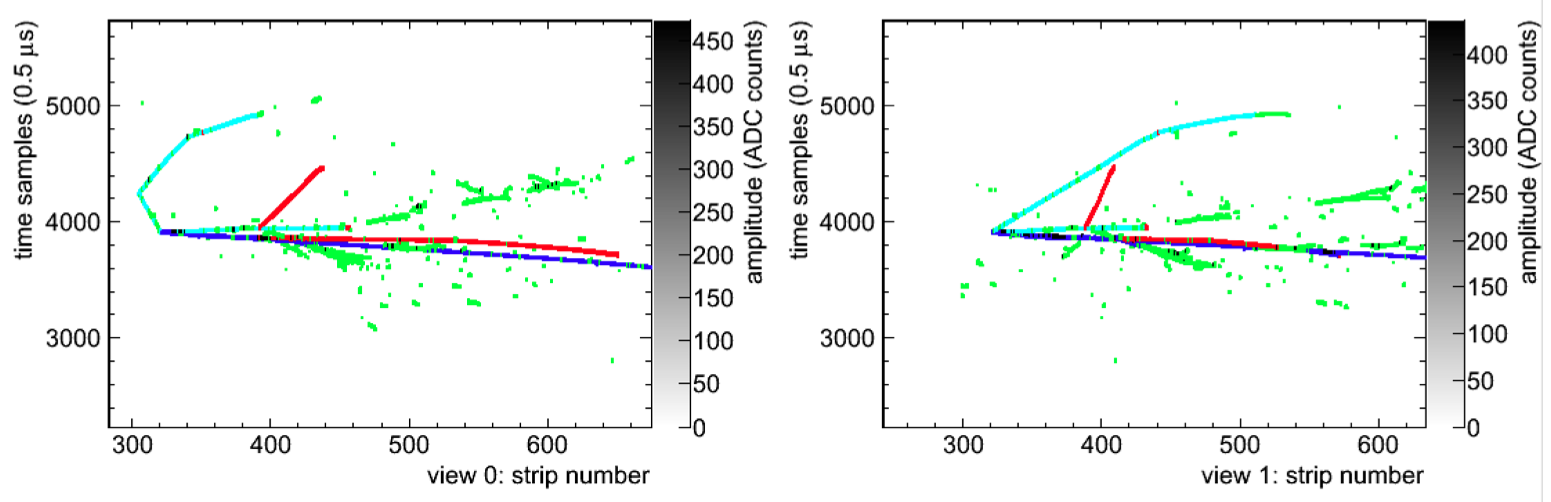
\includegraphics[width=0.99\textwidth]{LBNO-MC-nu_mu_event.png}
\end{cdrfigure}


The wrapping of induction-plane wires in the single-phase APA design
introduces an additional discrete ambiguity in the data by connecting
multiple wire segments to each DAQ channel. A ``disambiguation''
algorithm is used to break the ambiguity and determine which wire
segment generated the charge on each hit.  The algorithm forms
associations between the collection and induction views, identifying
``triplets'' of hits that have intersecting wire segments and
consistent arrival times. In most events, the majority of hits are
associated with a single wire segment, and can be trivially
disambiguated.  The remaining hits are then disambiguated by
clustering them with trivially disambiguated hits.

\subsubsection{Photon Detector Signal Reconstruction}

Photon detector signals are processed in similar ways to those on the
TPC wires.  Noise is filtered out, and hits are identified as pulses
above the pedestal.  Hits are grouped together into clusters in time,
called ``flashes,'' for subsequent association with clusters in the
TPC.  Each flash has a time, a total integrated charge, and a position
estimate.  The time of an interaction is important in order to help
reject cosmic-ray events and also to determine the absolute position
of an event along the drift direction.  This position is important in
order to correct for finite electron lifetime effects for proper
charge measurement, which is important for particle identification and
extraction of physics results.  Signal events which can be out of time
from the beam include atmospheric neutrinos, supernova burst
neutrinos, and proton decay interactions.

\subsubsection{TPC Pattern Recognition}

The reconstruction of particles in 3D can be accomplished either by
forming 2D clusters and associating them between views, or by first
associating 2D hits between views and then clustering the resulting 3D
hits.  The clustering of hits in LArTPC detectors is a challenging
task due to the variety and complexity of event topologies.  However,
several automated 2D and 3D pattern-recognition algorithms have been
implemented using a range of techniques.

One promising suite of reconstruction tools is the PANDORA software
development kit\cite{Marshall:2013bda,Marshall:2012hh} which provides
fully automated pattern recognition for both single-phase and
dual-phase technologies.  PANDORA implements a modular approach to
pattern recognition, in which events are reconstructed using a large
chain of algorithms.  Several 2D pattern-recognition algorithms are
first applied that cluster together nearby hits based on event
topology.  The resulting 2D clusters are then associated between views
and built into 3D tracks and showers, modifying the 2D clustering as
needed to improve the 3D consistency of the event.  Vertex-finding
algorithms are also applied, and neutrino events are reconstructed by
associating the 3D particles to the primary interaction vertex.

Figure~\ref{fig:pandoraefficiency} shows the current efficiency for
reconstructing the leading final-state lepton as a function of its
momentum for 5~GeV $\nu_{e}$ and $\nu_{\mu}$ charged-current
interactions simulated in the MicroBooNE detector; the DUNE
single-phase detector is expected to perform similarly, although the
multiple TPC geometry with wrapped wires requires additional software
effort.
%In both samples, the reconstruction efficiency increases rapidly with momentum,
%rising above 90\% at 500\,MeV and reaching approximately 100\% at 2\,GeV.
Figure~\ref{fig:recoannexpandoravertexresolution} shows the spatial
resolution for reconstructing the primary interaction vertex in these
5-GeV event samples, projected onto the $x$, $y$ and $z$ axes. An
estimate of the overall vertex resolution is obtained by taking the
68\% quantile of 3D vertex residuals, which yields 2.2~cm (2.5~cm)
for $\nu_{\mu}$CC ($\nu_{e}$CC) events.
\begin{cdrfigure}[PANDORA reconstruction efficiency]{pandoraefficiency}
{Reconstruction efficiency of Pandora pattern recognition algorithms
 for the leading final-state lepton in 5-GeV $\nu_{\mu}$ CC (left) and
 $\nu_{e}$ CC (right) neutrino interactions, plotted as a function of
 the lepton momentum. The reconstruction performance is evaluated
 using the MicroBooNE detector geometry. }
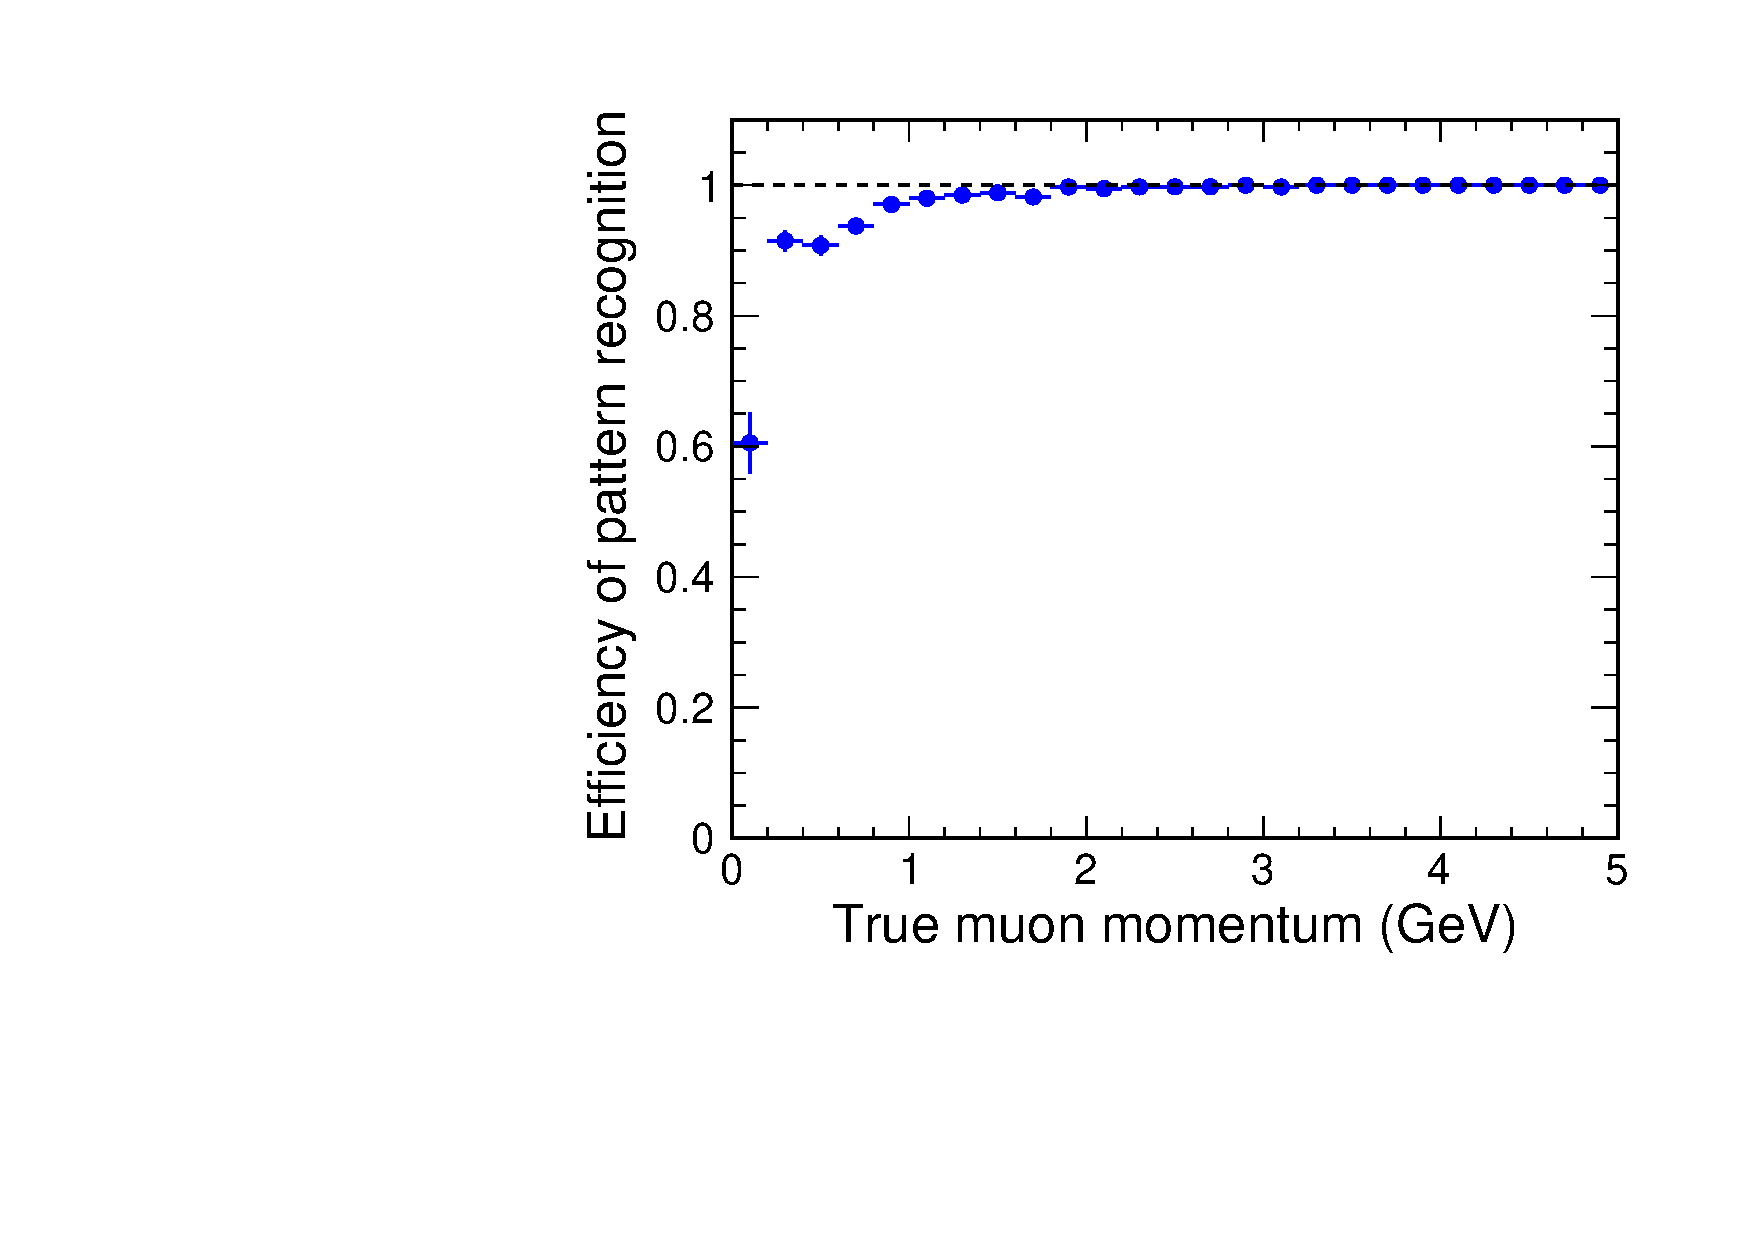
\includegraphics[width=0.49\textwidth]{pandora_uboone_efficiency_5GeV_numucc.pdf}
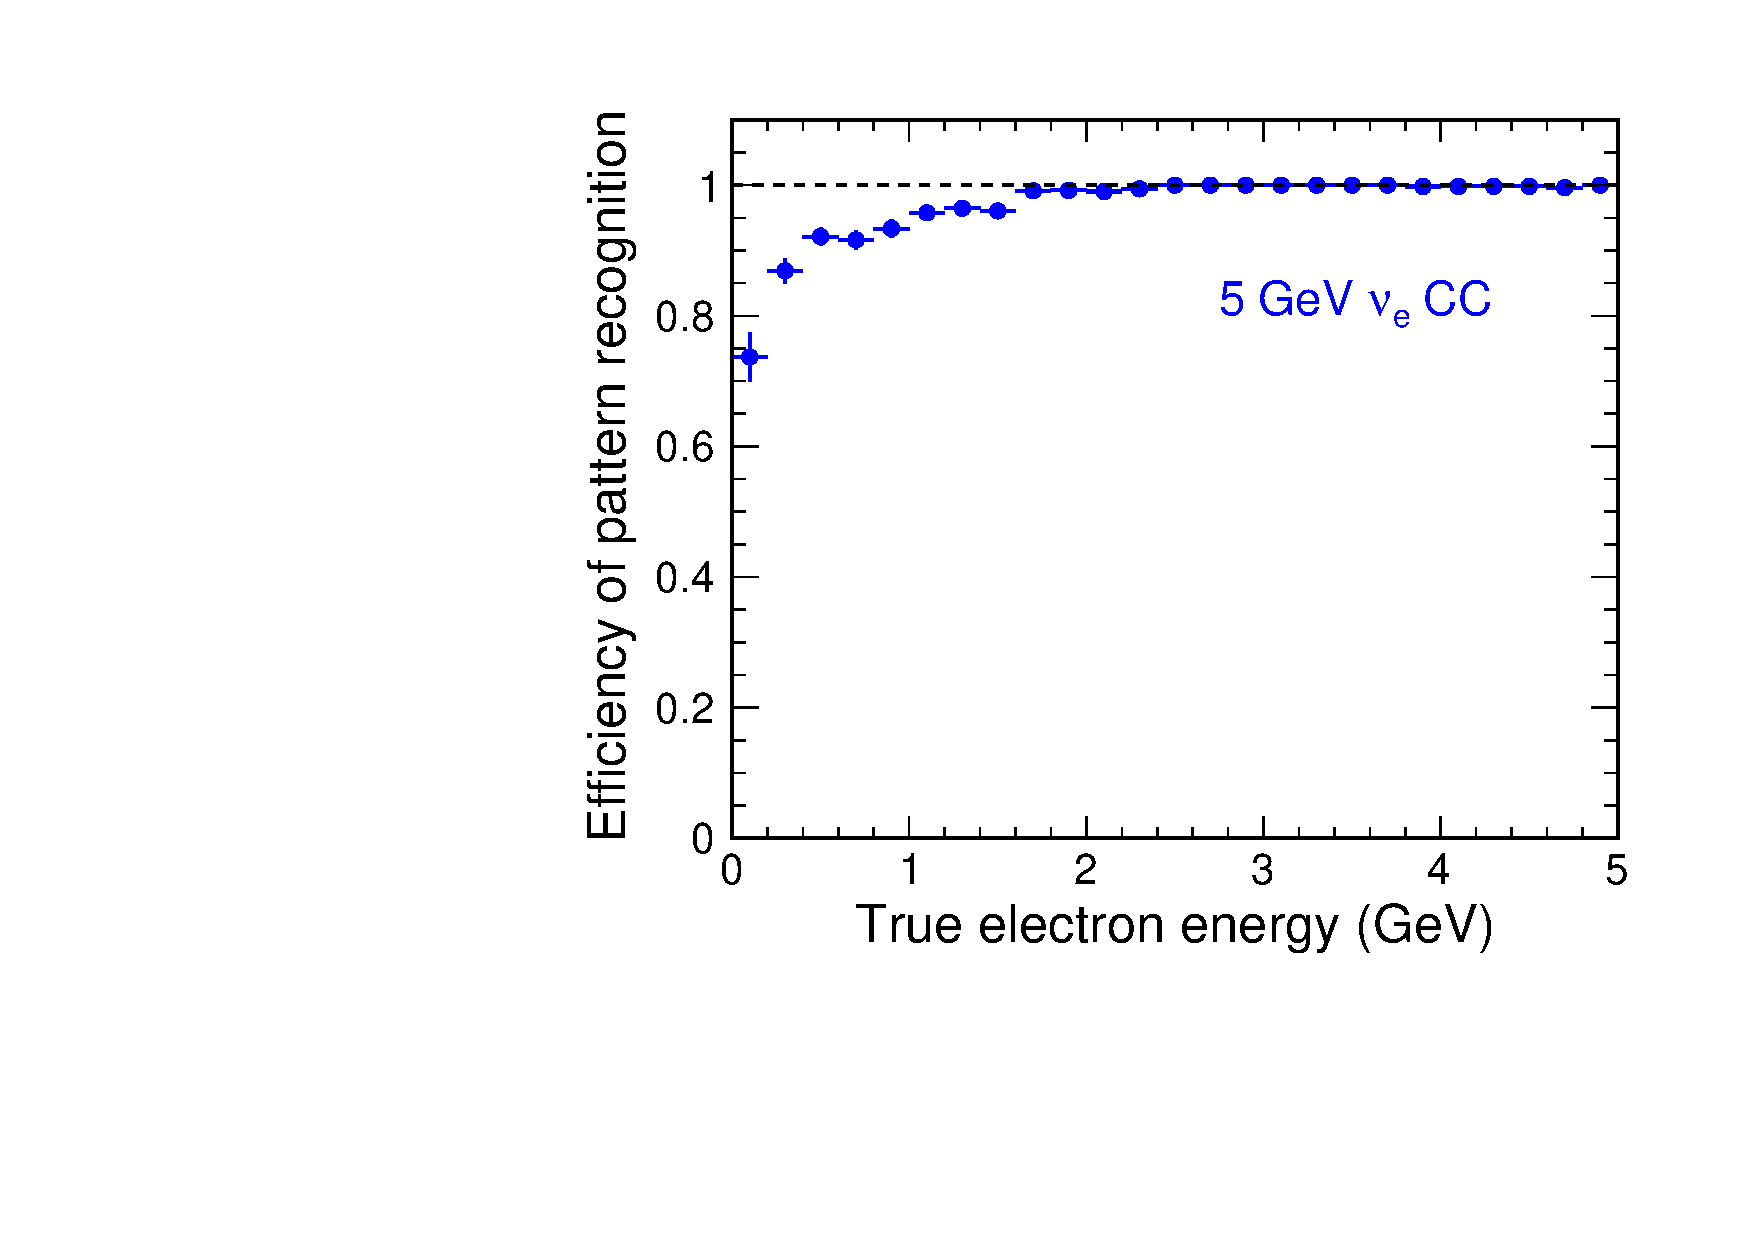
\includegraphics[width=0.49\textwidth]{pandora_uboone_efficiency_5GeV_nuecc.pdf}
\end{cdrfigure}
\begin{cdrfigure}[PANDORA vertex resolution]{recoannexpandoravertexresolution}
{Distribution of 2D residuals between reconstructed and simulated interaction
 vertex for 5-GeV $\nu_{\mu}$ CC (left) and $\nu_{e}$ CC (right) interactions in the MicroBooNE detector.
 The $x$ axis is oriented along the drift field, the $y$ axis runs parallel 
 to the collection plane wires, and the $z$ axis points along the beam direction.}
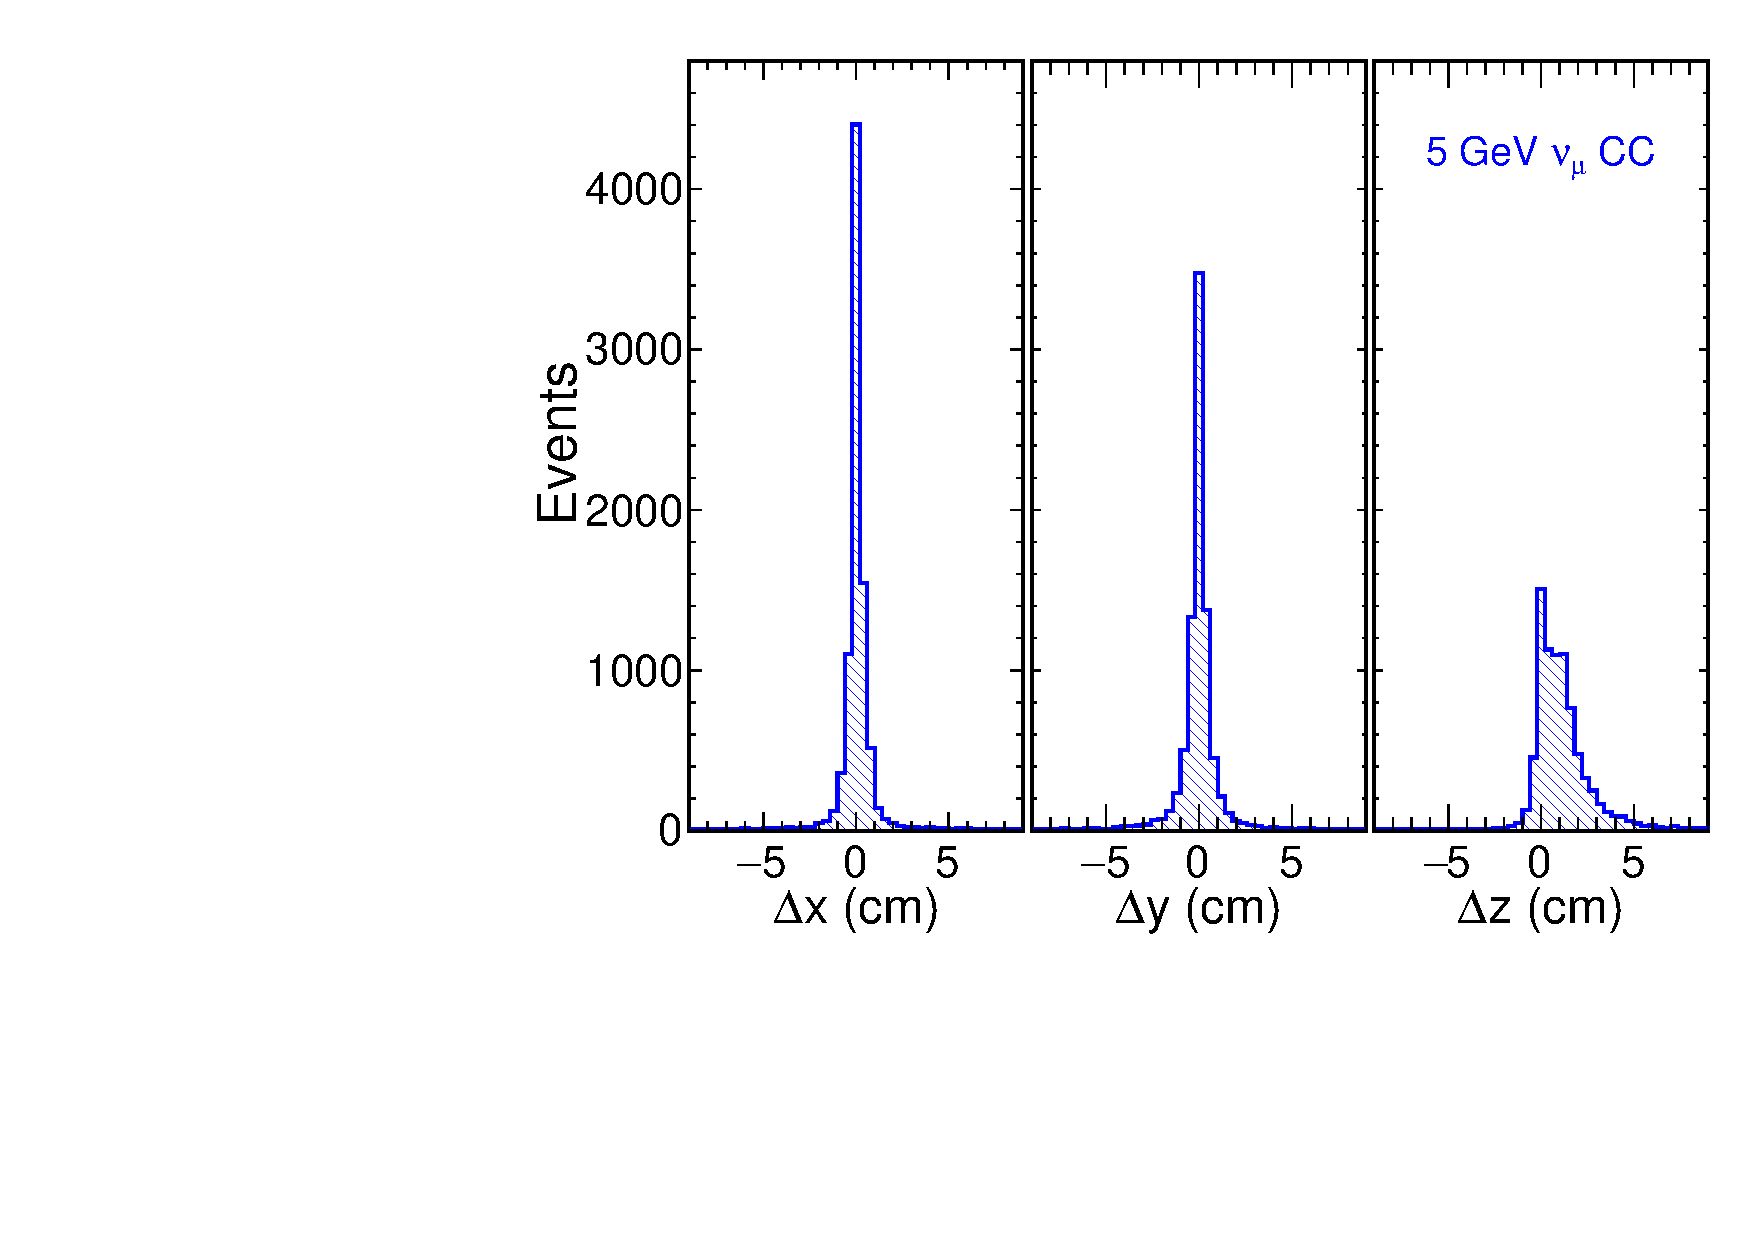
\includegraphics[width=0.49\textwidth]{pandora_uboone_vertex_resolution_numucc.pdf}
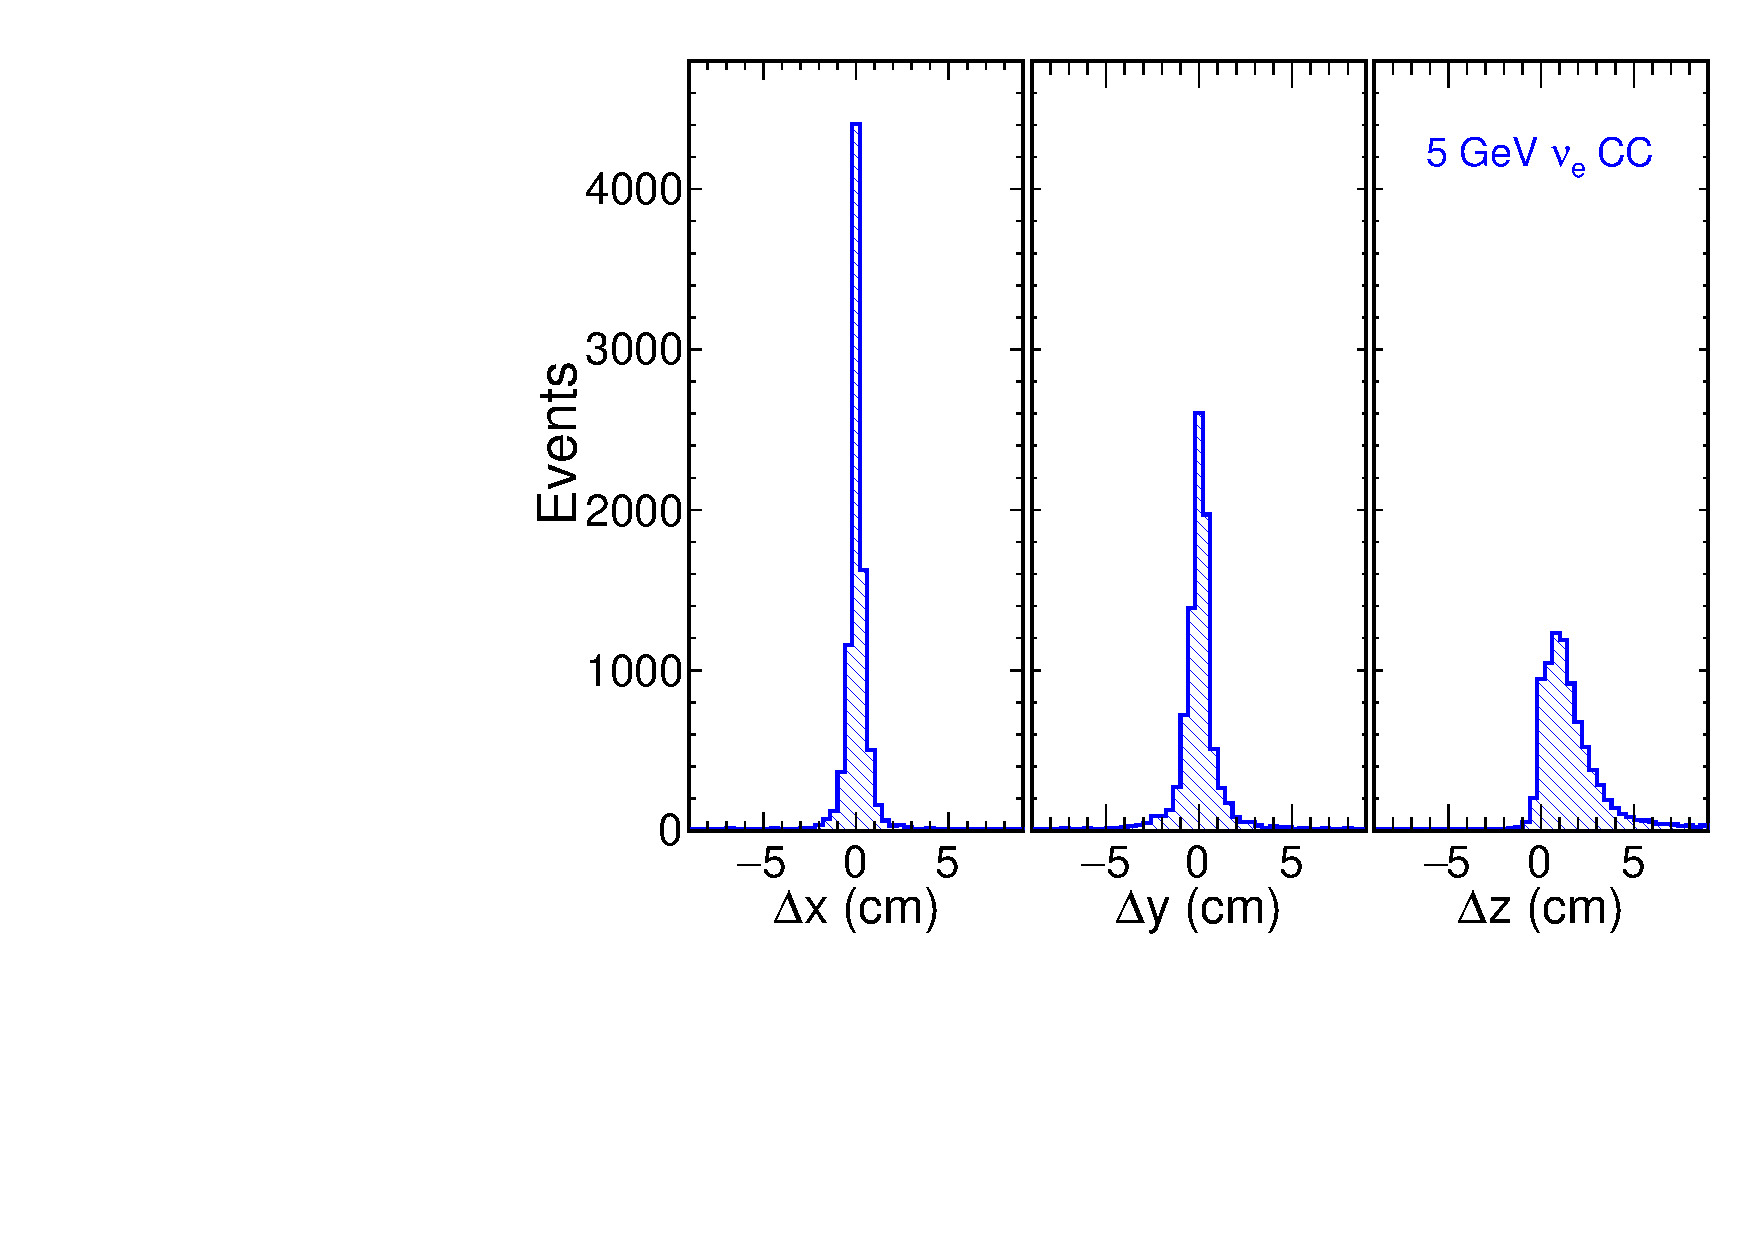
\includegraphics[width=0.49\textwidth]{pandora_uboone_vertex_resolution_nuecc.pdf}
\end{cdrfigure}

\subsubsection{Track Fitting and Shower Measurement}

After the pattern recognition stage, a series of high-level
reconstruction algorithms is applied to the 2D and 3D clusters, which
fit the trajectories of particle tracks and measure the spatial and
calorimetric properties of electromagnetic and hadronic showers.
Several high-level techniques have been demonstrated for use in LArTPC
detectors using both real and simulated data.

The Kalman filter technique\cite{kalman} is well-established in
high-energy physics, and has been applied to 3D track reconstruction
in liquid argon by ICARUS\cite{Ankowski:2006ts}.  The technique
incorporates the effects of multiple Coulomb scattering, enabling a
scattering-based measurement of the track momentum, which is shown by
ICARUS to have a resolution as good as $\Delta p/p \approx 10\%$ for
the most favourable track lengths.  The data from ICARUS have also
been used to develop a precise track reconstruction algorithm, which
builds a 3D trajectory for each track by simultaneously optimizing its
2D projections to match the observed data\cite{Antonello:2012hu}.
Another promising track reconstruction technique, based on the local
principal curve algorithm, has been implemented for the dual-phase
detector, and is shown to provide a precise reconstruction of two-body
final states~\cite{Back:2013cva,LAGUNA-LBNO-deliv}.

A full 3D reconstruction of electromagnetic showers is currently in
development.  In the present scheme, the first stage is an examination
of clusters in terms of their 2D parameters, and a selection of
shower-like clusters for further analysis. The 3D start position,
principal axis, and shower shape variables are then reconstructed by
matching up 2D hits between views.  These 3D parameters, combined with
calorimetric information, enable a measurement of the total shower
energy, as well discrimination between electrons and converted photons
based on the ionization energy in the initial part of the shower. The
kinematic reconstruction of final-state neutral pions from their
$\pi^{0} \rightarrow \gamma\gamma$ decays can be performed by
combining together associated pairs of photons.


\subsubsection{Calorimetry and Particle Identification}

The reconstructed energy of hits follows from the measured charge
after corrections are made for sources of charge loss.  The energy of
physics objects can then be reconstructed by summing the energy of the
associated hits and, when this is combined with reconstructed
trajectory, a measurement of the ionization density $dE/dx$ can be
made, which is an important input to particle identification.  In
order to reconstruct this information, the measured charge on each hit
is first obtained from fits to the pulse shapes.  The charge loss due
to the finite electron lifetime is corrected based on the time of the
event, and the path length corresponding to each hit is calculated
based on the event trajectory.  The effects of recombination, known as
``charge quenching'' are corrected using a modified Box
model\cite{Thomas:1987zz} or Birks Law\cite{Birks:1964zz}.  The
identity of a particle track that ranges out in the active detector
volume may be ascertained by analyzing the ionization density $dE/dx$
as a function of the range from the end of the track, and comparing
with the predictions for different particle species.

In a liquid argon TPC, electromagnetic showers may be classified as
having been initiated by an electron or a photon using the $dE/dx$ of
the initial $\sim$2.5~cm of the shower.  Electron-initiated showers
are expected to have $dE/dx$ of one MIP in the initial part, while
photon-initiated showers are expected to have twice that.  Current
algorithms achieve a performance of 80\% electron efficiency with 90\%
photon rejection, with a higher efficiency for fully-reconstructed
showers.

%Do we have any calorimetry plots?  
% not for the main CDR.  Perhaps the annex


\subsubsection{Neutrino Event Reconstruction and Classification}

Once the visible particles in an event have been reconstructed
individually, the combined information is used to reconstruct and
classify the overall event.  The identification of neutrino event
types is based on a multivariate
analysis\cite{Back:2013cva,WA105_TDR,LAGUNA-LBNO-deliv,LAGUNA-LBNO-EOI},
which constructs a number of characteristic topological and
calorimetric variables, based on the reconstructed final-state
particles. In the present scheme, a Boosted Decision Tree algorithm is
used to calculate signal and background likelihoods for particular
event hypotheses. The current performance has been evaluated using
fully reconstructed $\nu_{e}$ and $\nu_{\mu}$ charged-current
interactions with two-body final states, simulated in the dual-phase
far detector\cite{LAGUNA-LBNO-deliv}.  The correct hypothesis is
chosen for 92\% (79\%) of $\nu_{\mu}$ ($\nu_{e}$) quasi-elastic
interactions with a lepton and proton in the final state, and 79\%
(71\%) of $\nu_{\mu}$ ($\nu_{e}$) resonance interactions with a lepton
and charged pion in the final state.  For selected events, the
neutrino energy is estimated kinematically for quasi-elastic
interactions using a two-body approximation, or otherwise a
calorimetric energy measurement is applied.  The calorimetric
reconstruction takes into account the quenching factors of the
different particles, assuming that all hits not associated with the
primary lepton are due to hadronic activity.
Figure~\ref{fig:recoenergynue} shows the resulting energy
reconstruction for $\nu_e$ CCQE and CC1$\pi^{+}$ events.
\begin{cdrfigure}[Reconstruction of electron neutrino energy]{recoenergynue}
{Performance of neutrino energy measurement, evaluated using the dual-phase far detector simulation. 
Distributions of reconstructed versus true neutrino are shown for $\nu_{e}$ CCQE events (left),
assuming two-body kinematics, and $\nu_{e}$  CC1$\pi^{+}$ events (right),
using a calorimetric energy estimation.}
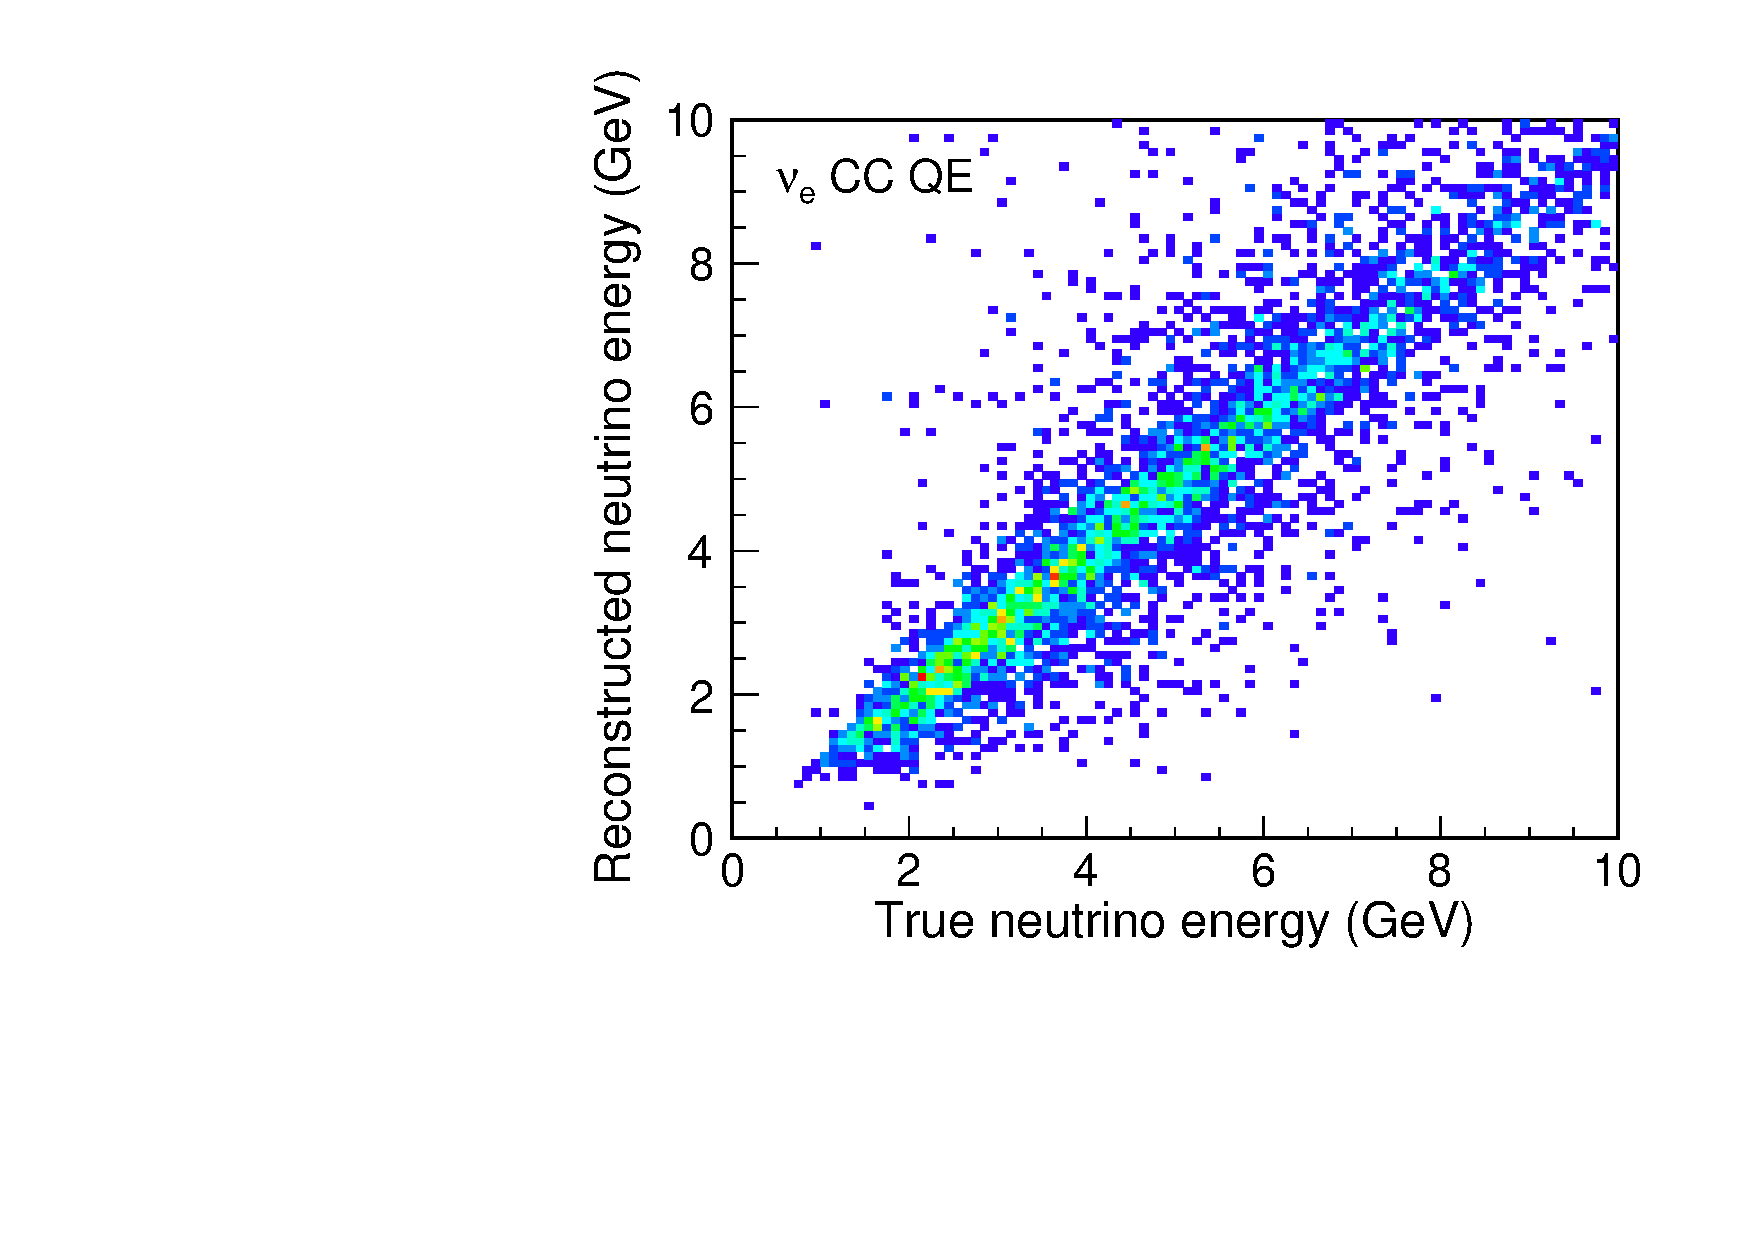
\includegraphics[width=0.49\textwidth]{laguna_lbno_recoenergy_nue_ccqe.pdf}
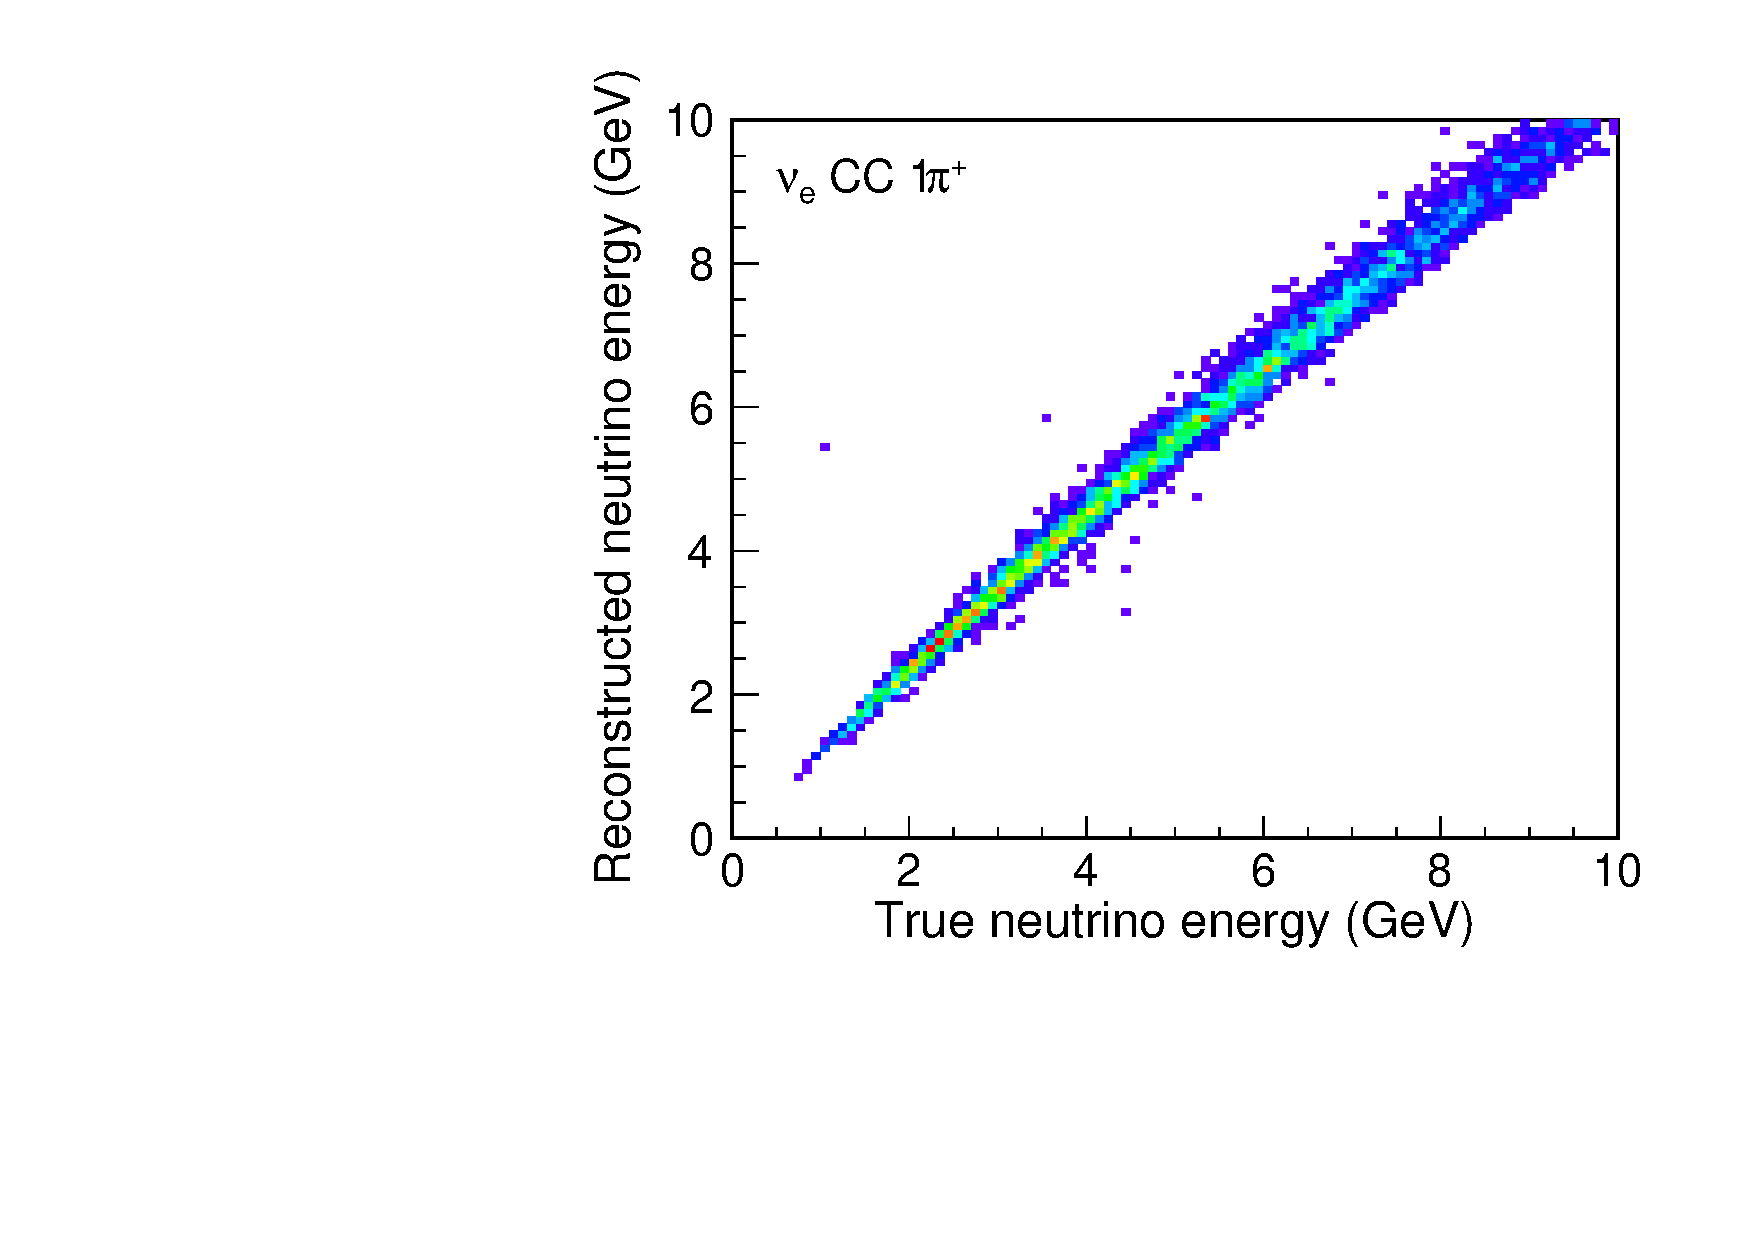
\includegraphics[width=0.49\textwidth]{laguna_lbno_recoenergy_nue_ccres.pdf}
\end{cdrfigure}

%%%% Do we need a summary?
% not really -- 5 pages is a little tight; this is the summary
